\title{Circuitos Eléctricos}
\maketitle
\section*{fuentes de tensión - ideal}
\justifying
Una fuente de tensión continua produce una tensión constante en la carga,	independientemente de lo grande o pequeña que sea la resistencia de carga.

Solo varia la corriente de carga cuando varia la resistencia de carga.

\begin{figure}[h]
	\centering
	\subfloat[Esquema]{
		\label{f:Esquema}
		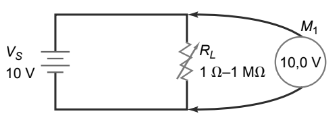
\includegraphics[width=0.2\textwidth]{f_t_c_esquema}}
	\subfloat[Grafica]{
		\label{f:Grafica}
		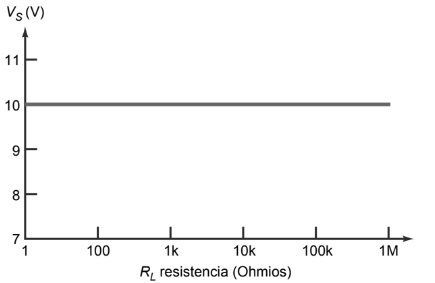
\includegraphics[width=0.2\textwidth]{f_t_c_grafica}}
	\label{f:Fuente de tension - Ideal}
\end{figure}

\section*{fuentes de tensión - real}
\justifying
Una fuente de tensión ideal es un dispositivo teórico; no puede existir en la naturaleza, porque cuando la resistencia de carga tiende a cero, la corriente por la carga tiende a infinito.

En este caso, la tensión en la carga no se aproxima al valor ideal hasta que la resistencia de
carga es mucho mayor que la resistencia de la fuente.

\centering{Fuente de tension continua $\rightarrow$ $R_s$ $<$ $0,01R_L$}

\section*{fuentes de corriente - ideal}
\justifying
Una fuente de corriente continua ideal, genera una corriente constante en la carga para distintas resistencias de carga

\section*{conversiones de fuentes}
\justifying
Es importante darse cuenta que la equivalencia entre una fuente de corriente y una fuente de tension existe solo en sus terminales externos.

Las caracteristicas internas de cada una son muy diferentes.

\section*{fuentes de corriente en paralelo}
\justifying
Dos o mas fuentes de corriente en paralelo pueden reemplazarse por una sola fuente de corriente de magnitud, determinada por la diferencia de la suma de la corrientes en una direccion y la suma en la direccion opuesta.

La nueva resistencia interna en paralelo es la resistencia total de los elementos resistivos en paralelo.
\section*{fuentes de corriente en serie}
\justifying
La corriente a traves de cada rama de una red solo puede tener un valor

Teniendo esto en cuenta, al conectar diferentes fuentes corriente en serie, la corriente que sale de un punto, sera diferente que la entra al otro, por lo cual es una situación imposible segun la Ley de Kirchhoff de las corrientes de un nodo.
\section*{divisor de corriente}
\section*{divisor de voltaje}
\section*{metodo de corriente de mallas}
\section*{metodo de voltajes de nodos}
\section*{teorema de superposicion}
\section*{teorema de thevenin}
\section*{teorema de norton}